% !TeX spellcheck = da_DK
\chapter{Android udvikling}

Når vi snakker om Android, så snakker vi om et "styresystem". Det kan man 
anskue som et kæmpe stort program, der administrerer alle de apps der kører på 
mobil-telefonen. I denne bog, bruger vi begreberne "styresystem" og "platform" 
i flæng.

De eneste relevante styresystemer til mobiler er, pt., de følgende to:

\begin{itemize}
	\item IOS (IPhone, IPads etc.)
	\item Android (Samsung, HTC, Sony etc.)
\end{itemize}

På SDC, kigger vi på den sidste af de to, nemlig Android platformen. Selvom 
app-udvikling til IOS og Android minder meget om hinanden, så er der en række 
væsentlige forskelle i de værktøjer man bruger. Derfor kigger vi kun på den ene 
af de to styresystemer.

\section{Hvad er Android apps?}

\marginfigure{xkcd_app.png}{Billede lånt af: \url{https://xkcd.com}}

Når man skal beskrive hvad en ``Android app'' er, så kan det gøres lidt 
simplere ved at forstå hvad en ``app'' er. App er en forkortelse for 
applikation, hvilket i denne kontekst er synonymt med ``et program''. Når vi 
snakker om en app, snakker vi derfor om et computer program, som er kodet med 
en række instruktioner. Derfor er de programmer du har på din mobil, som 
WordFeud, SnapChat og Facebook, alle eksempler på apps. Computerspil, som 
Farming Simulator 2017 og Battlefield 4 er faktisk også eksempler på apps, så 
det er faktisk et meget vidt begreb. 

I Android verdenen, er stort set alt apps. Lige fra låseskærmen og 
``indstillinger''-menuen til Super Mario Go, og Farmville. Derfor er der meget 
få grænser for hvad man kan opnå ved app-udvikling til Android.

\subsection{Anatomien af en Android app}
Android apps består af mange forskellige dele. De primære dele kan dog deles op i følgende tre kategorier:

\subsubsection{Ressourcer}
Ressourcer er indstillinger, billeder, layouts (se \autoref{sec:android:layouts}) og alt mulig andet data der bruges i en app. De findes i mappen \texttt{res/} og har forskellige undermapper, afhængig af hvilken type ressource det er.

\subsubsection{Activities}
Activities er aktiviteter man kan foretage sig i app'en. Der kan f.eks. være en "tag billede" activity, en "gem billedet" activity og en "se dit galleri af billeder" activity. Disse activities vil blive udforsket yderligere i \autoref{activities kapitel}.

\subsubsection{Manifest}
Et app-manifest er en beskrivelse af app'en som Android styresystemet gør brug af når den kører app'en på mobilen. I manifestet beskriver man hvilke rettigheder app'en har brug for, samt hvilke teknologier den gør brug af.

Derudover kan manifestet indeholde information om hvordan andre apps kan kommunikere med denne app, og andre indstillinger der binder app'en sammen med resten af platformen.

\section{Layouts}
\label{sec:android:layouts}

Layouts er en ressource som app'en gør brug af når den skal vise den 
\gls{interface}\footnote{En \gls{interface} er, i denne kontekst, det grafiske 
design som brugeren interagerer med. Det kan f.eks. være en menu med knapper 
eller et billede.} som brugeren skal se på inde i app'en. Det er en beskrivelse 
af strukturen i app'ens \gls{interface}.

For bedre at forstå layouts, skal vi først forstå den måde vi skriver et layout på. Ligesom med programmeringssprog, hvor vi har forskellige sprog til at beskrive kode på (som f.eks. Java), findes der forskellige måder at beskrive strukturer og layouts. Vi kalder disse sprog for \textit{strukturelle sprog}, en af de mere udbredte af sådanne sprog er det man kalder for \textit{XML}\footnote{e\textbf{X}tensible \textbf{M}arkup \textbf{L}anguage}.

\subsection{XML}
I sin kerne er XML et meget simpelt sprog. Det er bygget op af ``tags'', hvoraf 
der findes to slags tags: et ``opening-tag'' og et ``closing-tag''. 
Opening-tags er skrevet ved at have et ``mindre-end'' tegn ($<$), efterfulgt af 
noget tekst og så afsluttet med et ``større-end'' tegn ($>$). For eksempel, er 
følgende et opening-tag: \XmlInline|<Button>|.

Closing-tags er meget lig opening-tags, der er blot en skråstreg efter 
``mindre-end'' tegnet, for at indikere at dette tag lukker et opening-tag der 
er skrevet tidligere i dokumentet. Et eksempel på et closing-tag, der lukker 
det opening-tag der var i det tidligere eksempel, kan ses her: 
\XmlInline|</Button>|.

Det er vigtigt at man altid lukker sine tags. Man må aldrig have et opening-tag uden at det bliver lukket, og man må aldrig have et closing-tag der ikke har noget opening-tag at lukke.

Man kan tilknytte ``attributter'' til sine opening-tags. Det gør man ved at 
skrive navnet på attributten, efterfulgt af et lig-med tegn, efterfulgt af 
attributtens værdi. Denne værdi er typisk skrevet inden i to gåse-øjne ("). Et 
eksempel på et opening-tag med en attribut er følgende: 
\XmlInline|<Button Text="Hej med dig!">|.

Et eksempel på et XML dokument ses herunder. Det beskriver et vindue, med en 
``label'' dvs. et kort stykke tekst, med to knapper. Vi har skrevet de tags, 
der hører til vores label og knapperne, imellem vinduets opening- og 
closing-tags. Dette betyder at de kommer til at høre til vinduet, altså at 
vinduet har en label og to knapper. Denne relation bliver ofte beskrevet som at 
vinduet er forældreren til de tre børn (label og de to knapper).

\begin{example}
	\begin{XmlCode}{Et lille XML dokument}{first-valid-xml-document}
		<Window>
			<Label Text="Vil du lukke vinduet?"></Label>
			<Button Text="Ja"></Button>
			<Button Text="Nej"></Button>
		</Window>
	\end{XmlCode}
\end{example}


For at simplificere XML dokumentet, kan vi udnytte os af et så-kaldt 
self-closing tag. Altså et opening-tag der lukkes med det samme, uden man 
behøver at bruge et closing-tag. Dette skrives ved at putte en skrå-streg ind 
før ``større-end'' tegnet:

\begin{example}
	\begin{XmlCode}{Et lille XML dokument med self-closing tags}{self-closing-tags-dokument}
		<Window>
			<Label Text="Vil du lukke vinduet?"/>
			<Button Text="Ja"/>
			<Button Text="Nej"/>
		</Window>
	\end{XmlCode}
\end{example}

\begin{remark}
	Bemærk at vi ikke kunne bruge et self-closing tag til vores \XmlInline|<Window>| tag, fordi at det ikke skulle lukkes med det samme, da det skulle indeholde dets tre børn.
\end{remark}

Bemærk at vi ikke kunne bruge et self-closing tag til vores \XmlInline|<Window>| tag, fordi at det ikke skulle lukkes med det samme, da det skulle indeholde dets tre børn.

Vi har nu taget en kort intro til XML, det er faktisk et meget mere komplekst sprog end det vi har gennemgået her, men det burde ikke blive nødvendigt at forstå det hele for det vi skal arbejde med her.

Hvis man gerne vil lære mere om XML, kan man besøge W3Schools: \url{https://www.w3schools.com/xml/}.


\subsection{Hvad er layouts?}
Layouts er, som nævnt, en måde at beskrive app'ens udseende på igennem det strukturelle sprog XML.

Vi lægger layouts i ressource mappen \texttt{res/layout/}, og et layout er 
faktisk bare et XML-tag der kan indeholde andre tags. De beskriver hvordan 
flere visuelle elementer skal pladseres i forhold til hinanden.

I Android Studio er der mulighed for at arbejde med disse layouts igennem en 
visuel editor, så man slipper for at rode med XML-kode. Det er dog stadig en 
god idé at forstå hvordan de fungerer i koden, både for forståelsens skyld og 
for at kunne rette fejl hvis det visuelle redigeringsværktøj driller.

\subsubsection{Frame layouts}

Det første eksempel på et layout er det såkaldte \textit{frame layout}, det er et meget simeplt og effektivt layout der er designet til at pladsere et enkelt element et specifikt sted på skærmen.

Det er svært at håndtere dette layout hvis det har mere end et barn. Derfor bør 
det typisk kun indeholde et enkelt barn. Deraf kommer navnet ``frame'', det 
bruges som en ``ramme'' til et andet element.

I \autoref{fig:android:layouts:frame-layout} er der et eksempel på hvordan man 
kan have to ``børn'' indeni et frame layout, for at placere det ene oven på det 
andet.

\begin{figure}[h]
	\begin{center}
		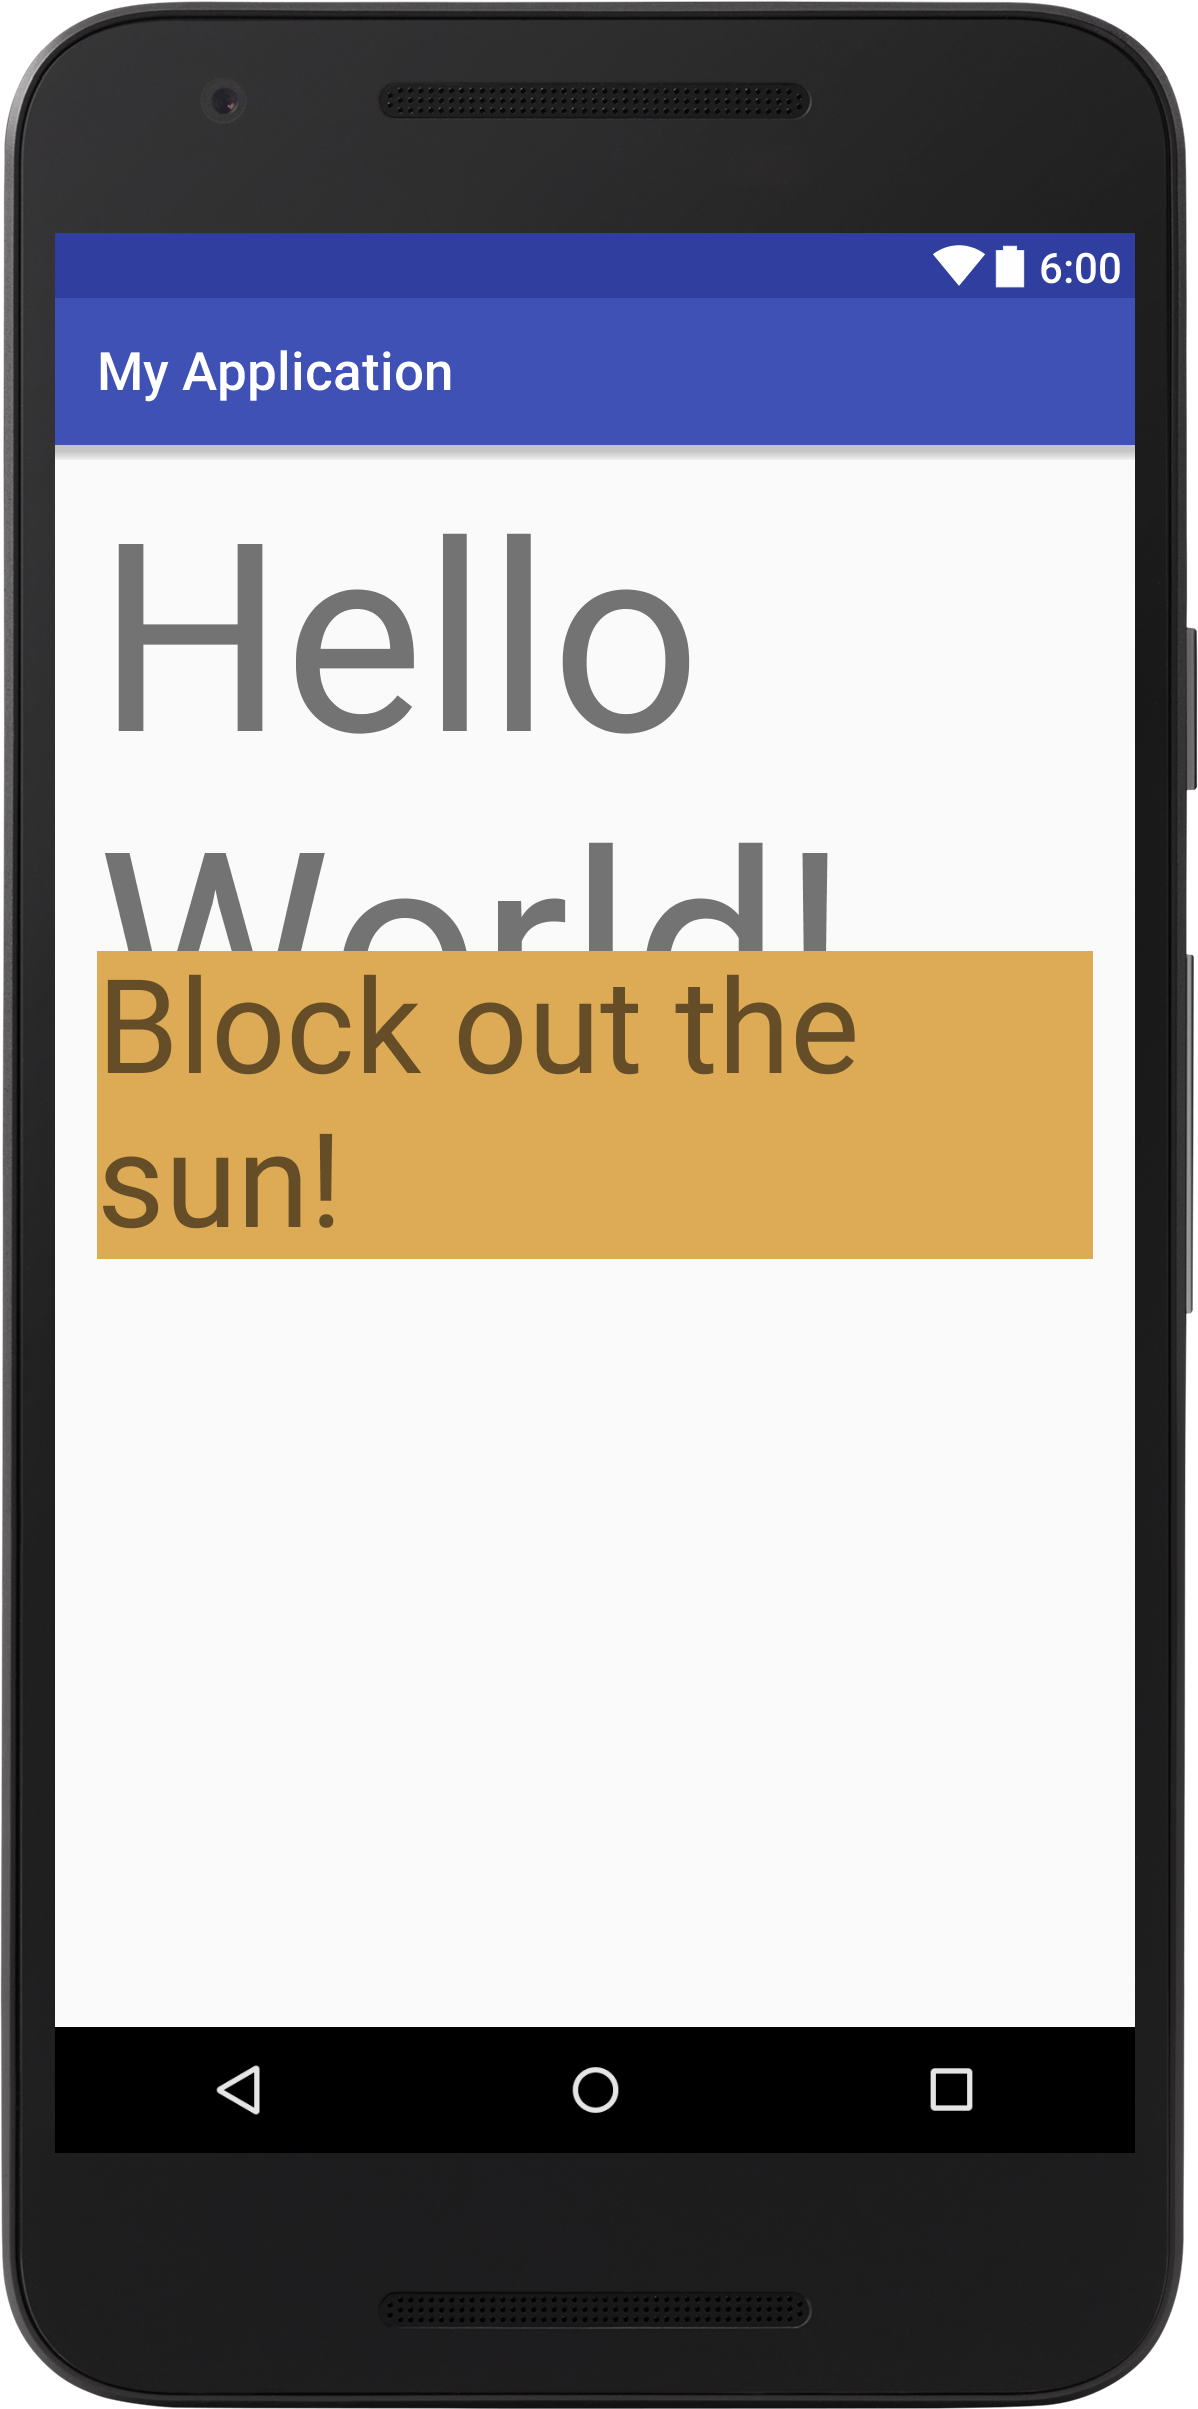
\includegraphics[width=5cm]{frame_layout.png}
		\caption{Et frame layout i en app}
		\label{fig:android:layouts:frame-layout}
	\end{center}
\end{figure}

\clearpage

\begin{XmlCode}{Det layout der giver udseendet i \autoref{fig:android:layouts:frame-layout}}{frame-layout}
	<?xml version="1.0" encoding="utf-8"?>
	<FrameLayout 
		xmlns:android=
			"http://schemas.android.com/apk/res/android"
		xmlns:tools="http://schemas.android.com/tools"
		android:layout_width="match_parent"
		android:layout_height="match_parent"
		android:paddingBottom=
			"@dimen/activity_vertical_margin"
		android:paddingLeft=
			"@dimen/activity_horizontal_margin"
		android:paddingRight=
			"@dimen/activity_horizontal_margin"
		android:paddingTop=
			"@dimen/activity_vertical_margin"
		tools:context=
			"com.example.lukas.myapplication.MainActivity">
	
		<TextView
			android:layout_width="wrap_content"
			android:layout_height="wrap_content"
			android:text="Hello World!"
			android:textSize="100sp"/>
		<TextView
			android:layout_width="fill_parent"
			android:layout_height="wrap_content"
			android:layout_gravity="center_vertical"
			android:layout_marginBottom="50dp"
			android:background="#ddaa55"
			android:text="Block out the sun!"
			android:textSize="50sp"/>
	</FrameLayout>
\end{XmlCode}

\subsubsection{Linear layouts}
Lineære layouts er det simpleste layout man kan bruge. Det tager alle sine 
børn, og arrangere dem således at de ligger enten under hinanden (vertikalt) 
eller ved siden af hinanden (horisontalt).

Der er ikke meget der kan ændres på hvordan dette layout virker, men det er 
rigtig simpelt til at vise f.eks. lister eller at pladsere elementer ved siden 
af hinanden.

I \autoref{fig:android:layouts:linear-layout} er der et eksempel på et lineært 
layout med tre børn, det første er bare sat ind og ligger øverst. Det næste er 
sat til at være lige så bredt som skærmen, og bliver automatisk sat nedenunder 
det første. Til sidst fylder det nederste og sidste element resten af skærmen.

\begin{figure}[h]
	\begin{center}
		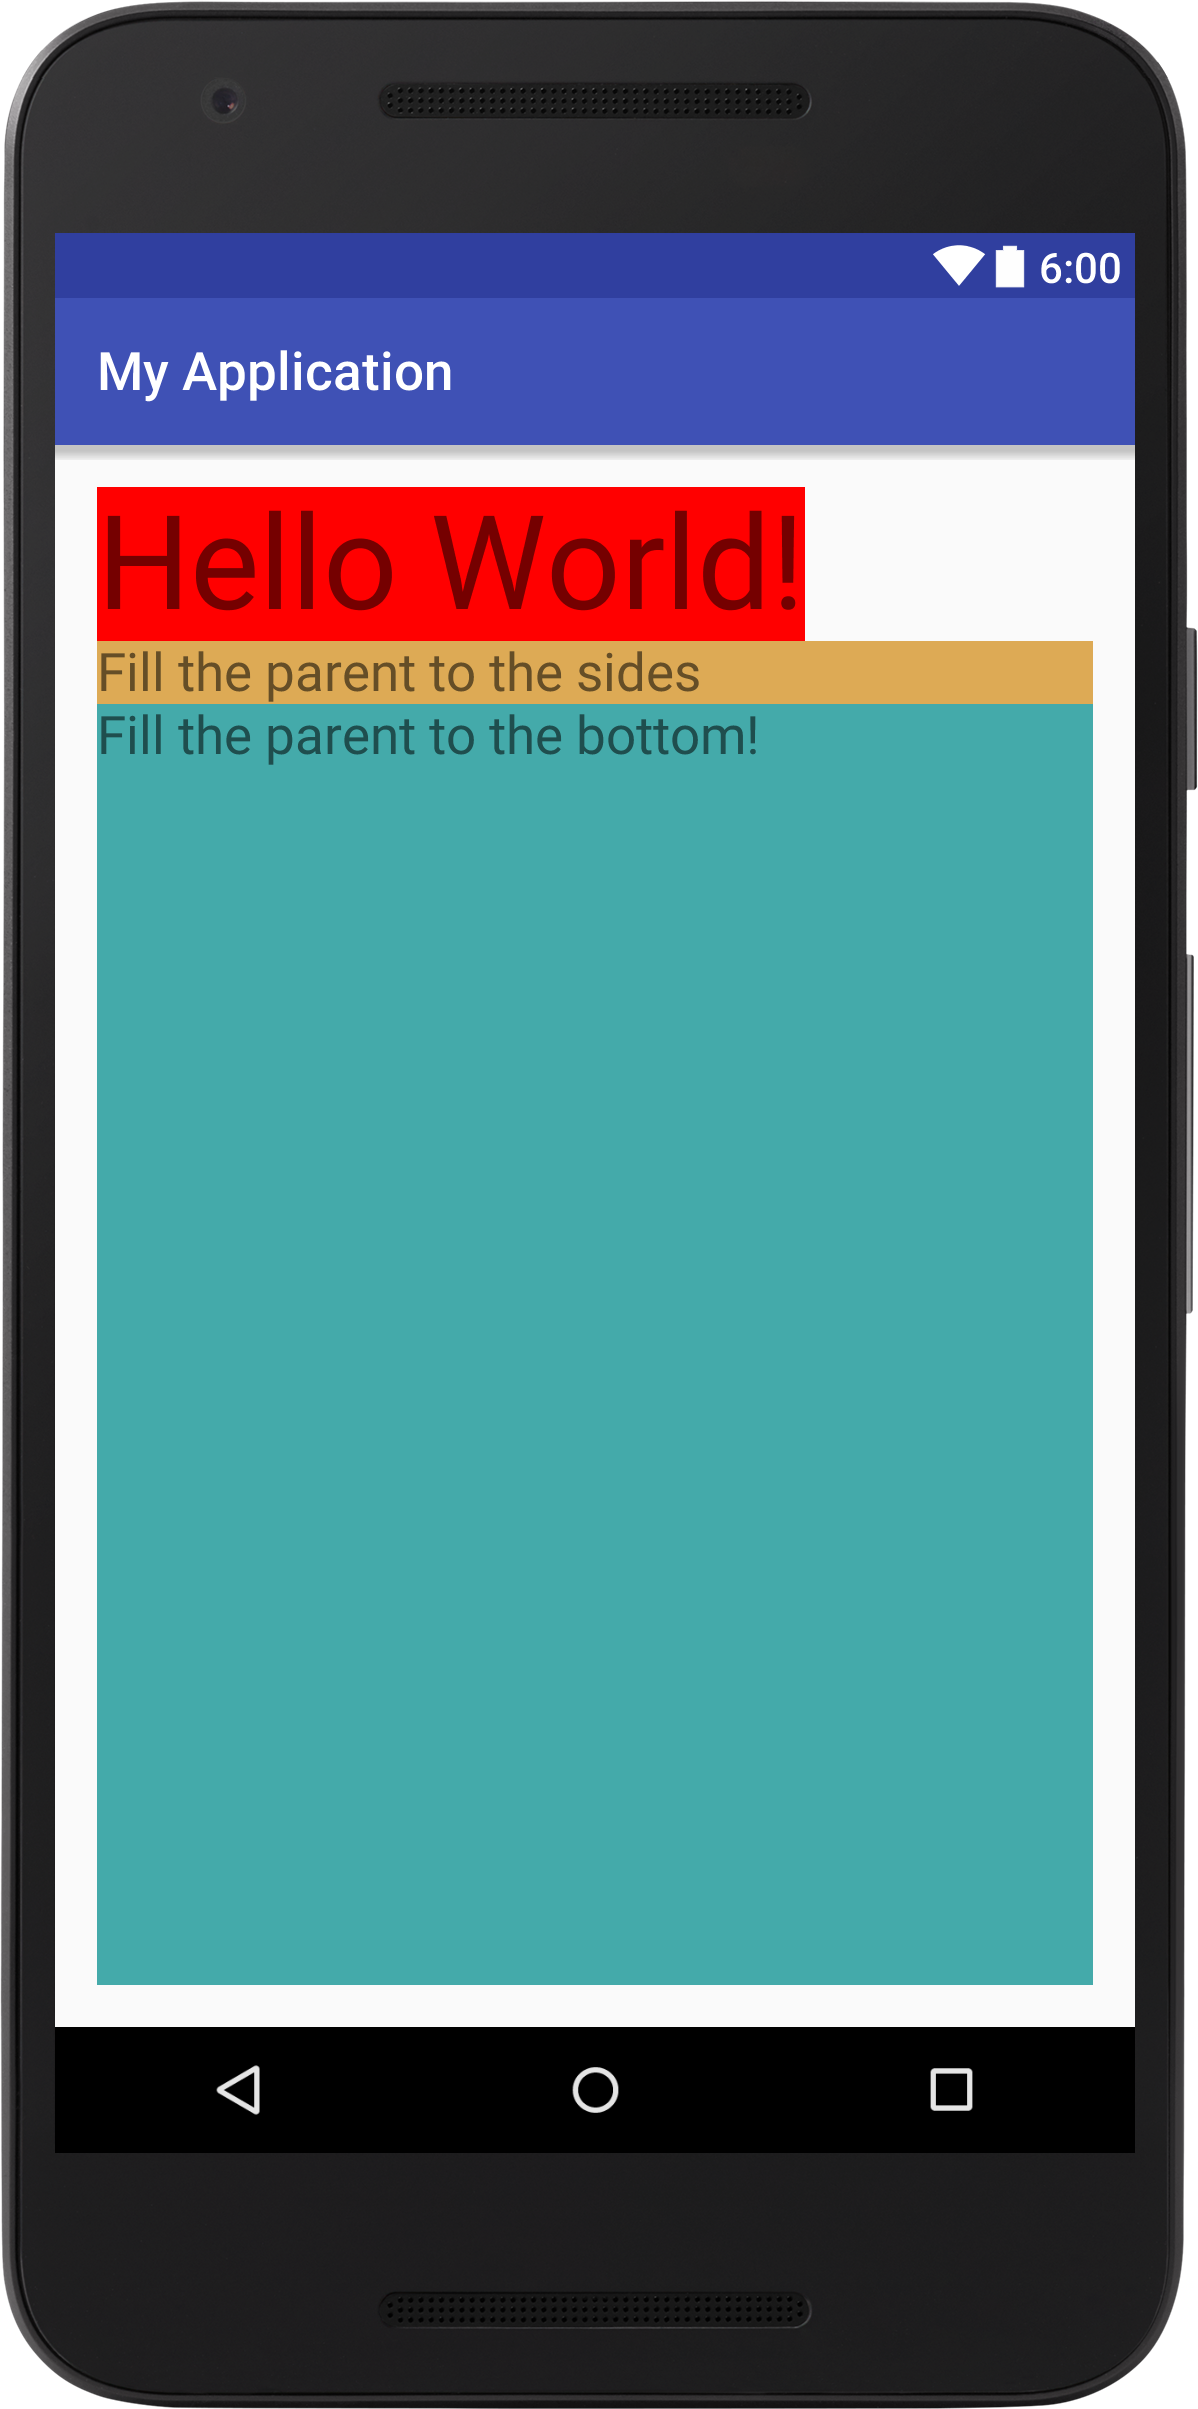
\includegraphics[width=5cm]{linear_layout.png}
		\caption{Et lineært layout i en app}
		\label{fig:android:layouts:linear-layout}
	\end{center}
\end{figure}

\clearpage

\begin{XmlCode}{Det layout der giver udseendet i %
\autoref{fig:android:layouts:linear-layout}}{linear-layout}
	<?xml version="1.0" encoding="utf-8"?>
	<LinearLayout 
		xmlns:android=
			"http://schemas.android.com/apk/res/android"
		xmlns:tools="http://schemas.android.com/tools"
		android:layout_width="match_parent"
		android:layout_height="match_parent"
		android:orientation="vertical"
		android:paddingBottom=
			"@dimen/activity_vertical_margin"
		android:paddingLeft=
			"@dimen/activity_horizontal_margin"
		android:paddingRight=
			"@dimen/activity_horizontal_margin"
		android:paddingTop=
			"@dimen/activity_vertical_margin"
		tools:context=
			"com.example.lukas.myapplication.MainActivity">
		
		<TextView
			android:layout_width="wrap_content"
			android:layout_height="wrap_content"
			android:text="Hello World!"
			android:background="#FF0000"
			android:textSize="50sp"/>
		<TextView
			android:layout_width="fill_parent"
			android:layout_height="wrap_content"
			android:background="#ddaa55"
			android:text="Fill the parent to the sides"
			android:textSize="20sp"/>
		<TextView
			android:layout_width="fill_parent"
			android:layout_height="fill_parent"
			android:layout_gravity="center_vertical"
			android:background="#44aaaa"
			android:text="Fill the parent to the bottom!"
			android:textSize="20sp"/>
	</LinearLayout>
\end{XmlCode}

\clearpage

\subsubsection{Table layouts}
Table layouts arrangerer sine børn i rækker og kolonner. De er simple og 
bruge, og er rigtig gode hvis man skal have noget der ligner en tabel men de er 
meget rigide. Alt man laver med tabular-layout vil se ud som en tabel.
 
 
I \autoref{fig:android:layouts:table-layout} er der et eksempel på et table 
layout. Der er 3 rækker og 3 kolonner i layoutet. Man laver nye rækker ved at 
putte det der skal være i rækken inden i et ``TableRow'' tag.
 
\begin{figure}[h]
	\begin{center}
		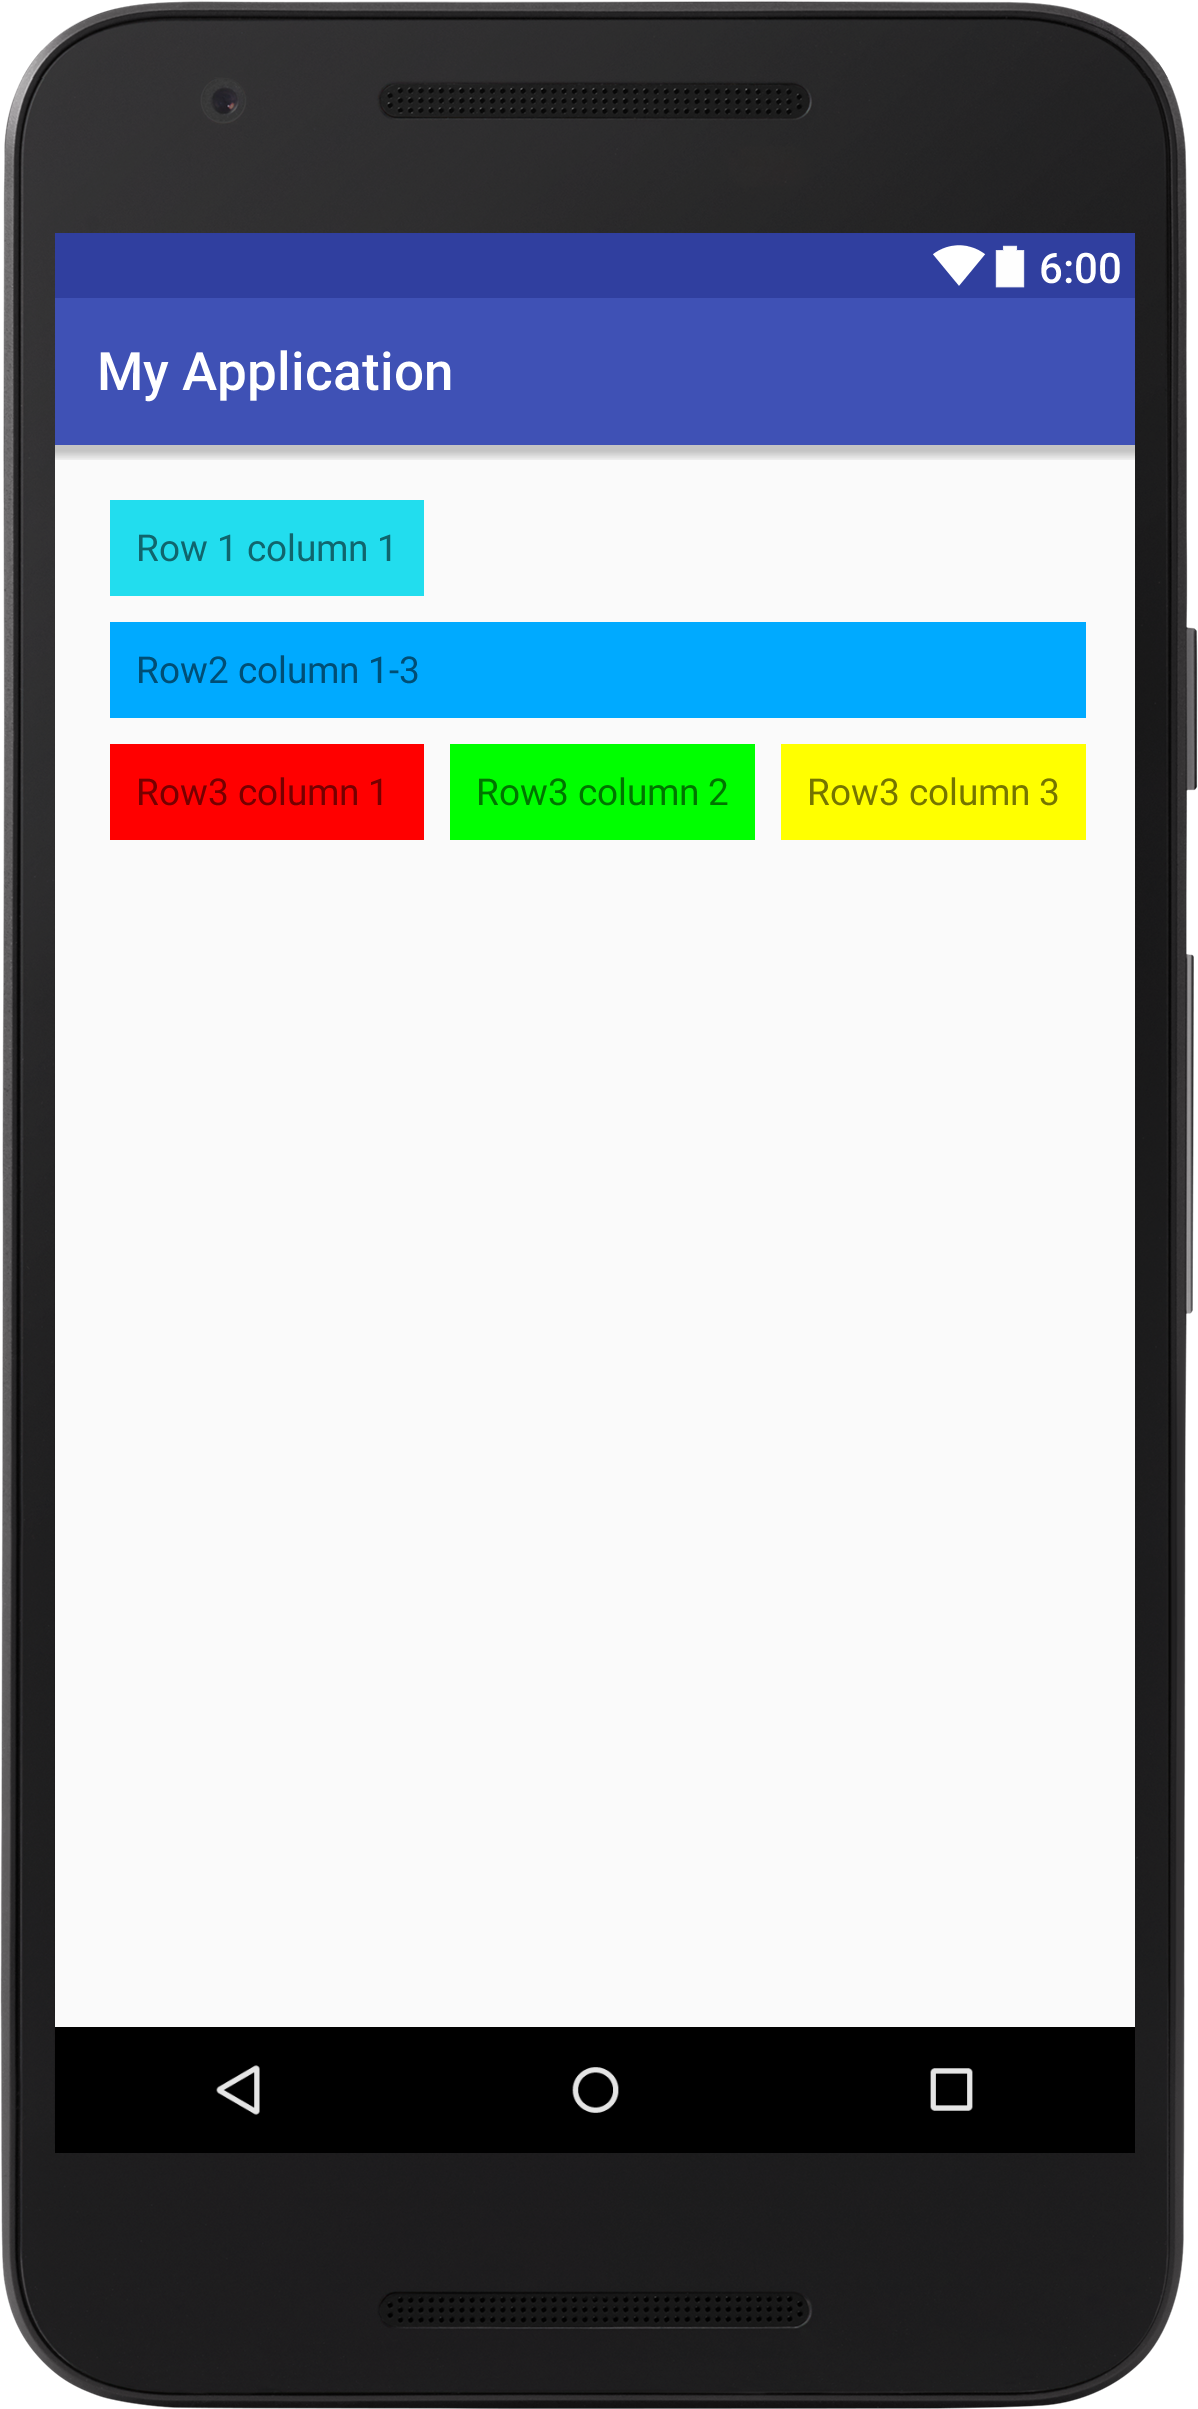
\includegraphics[width=5cm]{table_layout.png}
		\caption{Et table layout i en app}
		\label{fig:android:layouts:table-layout}
	\end{center}
\end{figure}
 
\clearpage
 
\begin{XmlCode}{Det layout der giver udseendet i %
 		\autoref{fig:android:layouts:table-layout}}{linear-layout}
	<?xml version="1.0" encoding="utf-8"?>
	<TableLayout 
		xmlns:android=
			"http://schemas.android.com/apk/res/android"
		xmlns:tools=
			"http://schemas.android.com/tools"
		android:layout_width="match_parent"
		android:layout_height="match_parent"
		android:paddingBottom=
			"@dimen/activity_vertical_margin"
		android:paddingLeft=
			"@dimen/activity_horizontal_margin"
		android:paddingRight=
			"@dimen/activity_horizontal_margin"
		android:paddingTop=
			"@dimen/activity_vertical_margin"
		tools:context=
			"com.example.lukas.myapplication.MainActivity">
		
		<TableRow>
			<TextView
			android:text="Row 1 column 1"
			android:background="#22ddee"
			android:padding="10dp"
			android:layout_margin="5dp"/>
		</TableRow>
		
		<TableRow>
			<TextView
			android:text="Row2 column 1-3"
			android:background="#00AAFF"
			android:padding="10dp"
			android:layout_span="3"
			android:layout_margin="5dp"/>
		</TableRow>
		
		<TableRow>
			<TextView
			android:text="Row3 column 1"
			android:background="#FF0000"
			android:padding="10dp"
			android:layout_margin="5dp"/>
			<TextView
			android:text="Row3 column 2"
			android:background="#00FF00"
			android:padding="10dp"
			android:layout_margin="5dp"/>
			<TextView
			android:text="Row3 column 3"
			android:background="#FFFF00"
			android:padding="10dp"
			android:layout_margin="5dp"/>
		</TableRow>
	</TableLayout>
\end{XmlCode}

\clearpage

\begin{exercise}
	Lav et tabular-lignende layout ved hjælp af linear layouts.
\end{exercise}

\begin{exercise}
	Lav et linear-lignende layout ved hjælp af tabular layouts (både horisontalt og vertikalt).
\end{exercise}

\subsubsection{Relative layouts}
Relative layouts er et meget fleksibelt og stærkt værktøj. De kan arrangere 
deres børn relativt til hinanden. F.eks. får man mulighed for at sige ``den 
røde kasse skal være til højre for den blå kasse''. Der er næsten ikke det man 
ikke kan med relative layouts.

\begin{figure}[h]
	\begin{center}
		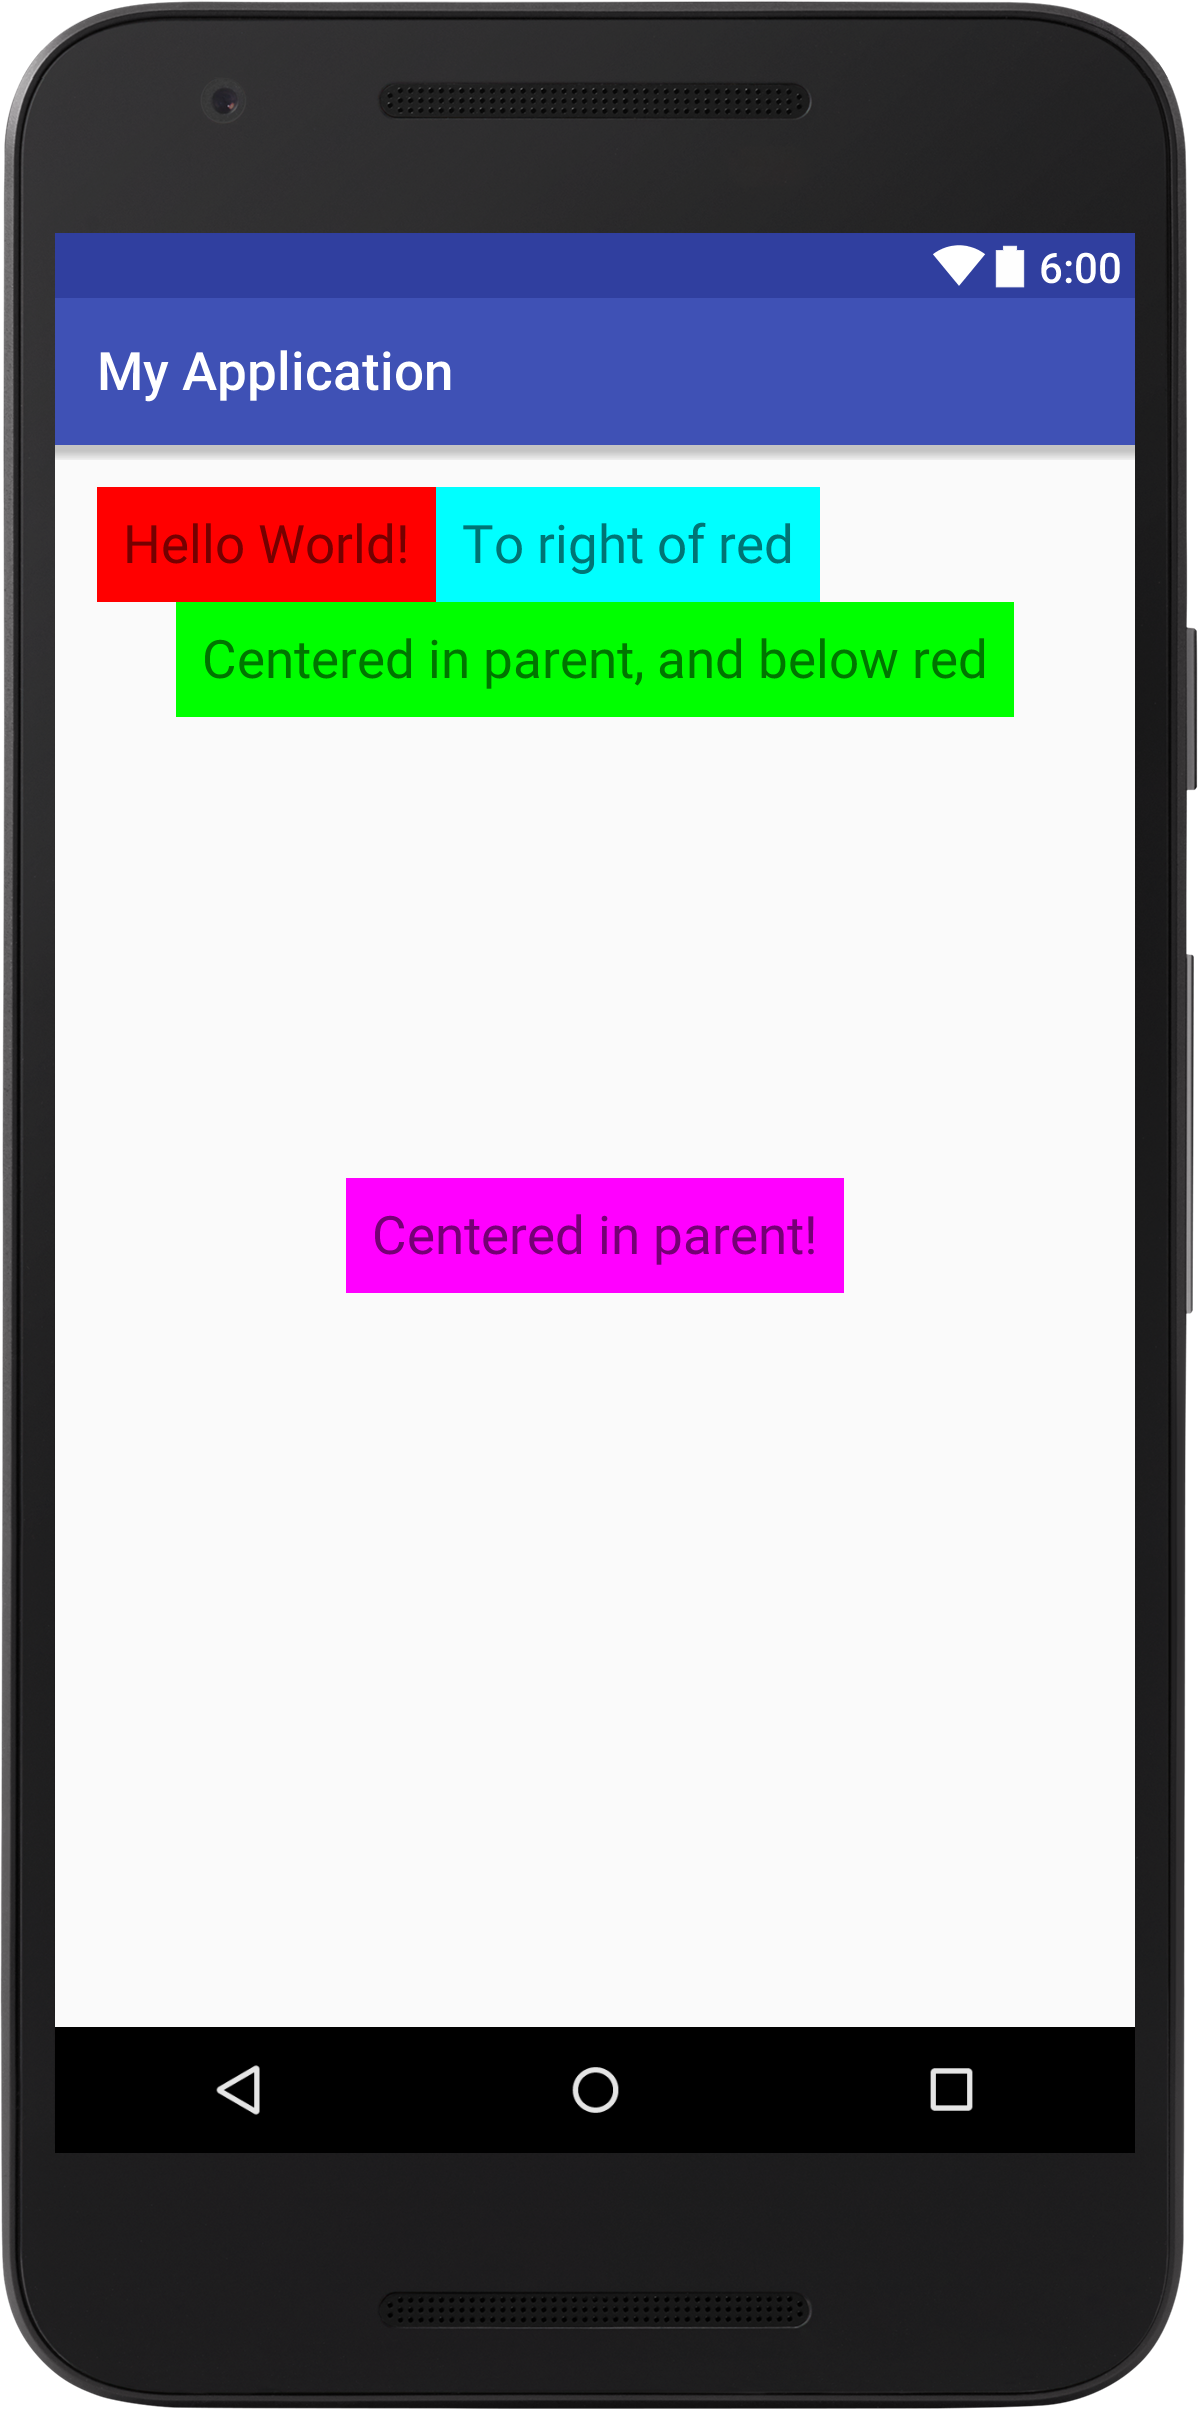
\includegraphics[width=5cm]{relative_layout.png}
		\caption{Et relative layout i en app}
		\label{fig:android:layouts:relative-layout}
	\end{center}
\end{figure}

\clearpage

\begin{XmlCode}{Det layout der giver udseendet i %
		\autoref{fig:android:layouts:relative-layout}}{relative-layout}
	<?xml version="1.0" encoding="utf-8"?>
	<RelativeLayout 
		xmlns:android=
			"http://schemas.android.com/apk/res/android"
		xmlns:tools=
			"http://schemas.android.com/tools"
		android:layout_width="match_parent"
		android:layout_height="match_parent"
		android:paddingBottom=
			"@dimen/activity_vertical_margin"
		android:paddingLeft=
			"@dimen/activity_horizontal_margin"
		android:paddingRight=
			"@dimen/activity_horizontal_margin"
		android:paddingTop=
			"@dimen/activity_vertical_margin"
		tools:context=
			"com.example.lukas.myapplication.MainActivity">
		
		<TextView
			android:id="@+id/text1"
			android:layout_width="wrap_content"
			android:layout_height="wrap_content"
			android:text="Hello World!"
			android:textSize="20dp"
			android:padding="10dp"
			android:background="#FF0000"
			android:layout_toRightOf="@id/text1"/>
		<TextView
			android:layout_width="wrap_content"
			android:layout_height="wrap_content"
			android:text="Centered in parent, and below red"
			android:textSize="20dp"
			android:padding="10dp"
			android:background="#00FF00"
			android:layout_below="@id/text1"
			android:layout_centerInParent="true"/>
		<TextView
			android:layout_width="wrap_content"
			android:layout_height="wrap_content"
			android:text="Centered in parent!"
			android:textSize="20dp"
			android:padding="10dp"
			android:background="#FF00FF"
			android:layout_centerInParent="true"/>
		<TextView
			android:layout_width="wrap_content"
			android:layout_height="wrap_content"
			android:text="To right of red"
			android:textSize="20dp"
			android:padding="10dp"
			android:background="#00FFFF"
			android:layout_toRightOf="@id/text1"/>
	</RelativeLayout>
\end{XmlCode}

\cleardoublepage

\section{Listeners}
I Android app-udvikling finder der noget der hedder en ``listener'', som navnet 
antyder så er der tale om noget der lytter. I app'ens \gls{interface}, er der 
tale om elementer der lytter efter brugerens input. F.eks. hvis man gerne vil 
skrive noget kode der reagerer på at brugeren trykker på en knap, er der tale 
om en ``On-Click-Listener''.

Disse listeners er altså måden hvorpå vi kan knytte vores \gls{interface} 
sammen med den kode vi gerne vil køre. Indtil videre har vi kun snakket om 
layouts, hvordan de virker og ser ud. I praksis er et layout næsten altid 
knyttet sammen med en Activity, som vi snakker mere om i 
\autoref{cha:activities-intents}. Lad os indtil videre antage at der kun er et 
layout (activity\_main.xml) og en activity (MainActivity.java). Hvis vi ikke 
har ændret i vores Activity, men blot bruger den Activity som Android Studio 
har lavet til os, vil koden se således ud:

\begin{JavaCode}{En tom MainActivity}{main-activity}
	public class MainActivity extends AppCompatActivity {
		
		@Override
		protected void onCreate(Bundle savedInstanceState) {
			super.onCreate(savedInstanceState);
			setContentView(R.layout.activity_main);
		}
	
	}
\end{JavaCode}

Læg mærke til dette stykke kode: 
\JavaInline|setContentView(R.layout.activity_main)|. I den linje knytter vi 
vores layout (activity\_main.xml) sammen med vores MainActivity, ved at sætte 
MainActivity's indhold til at være activity\_main layoutet.

Vi kan nu ændre vores activity\_main layout, ved at tilføje en knap i midten af 
skærmen, som vist i \autoref{fig:android:layouts:button-layout}.

\begin{figure}[h]
	\begin{center}
		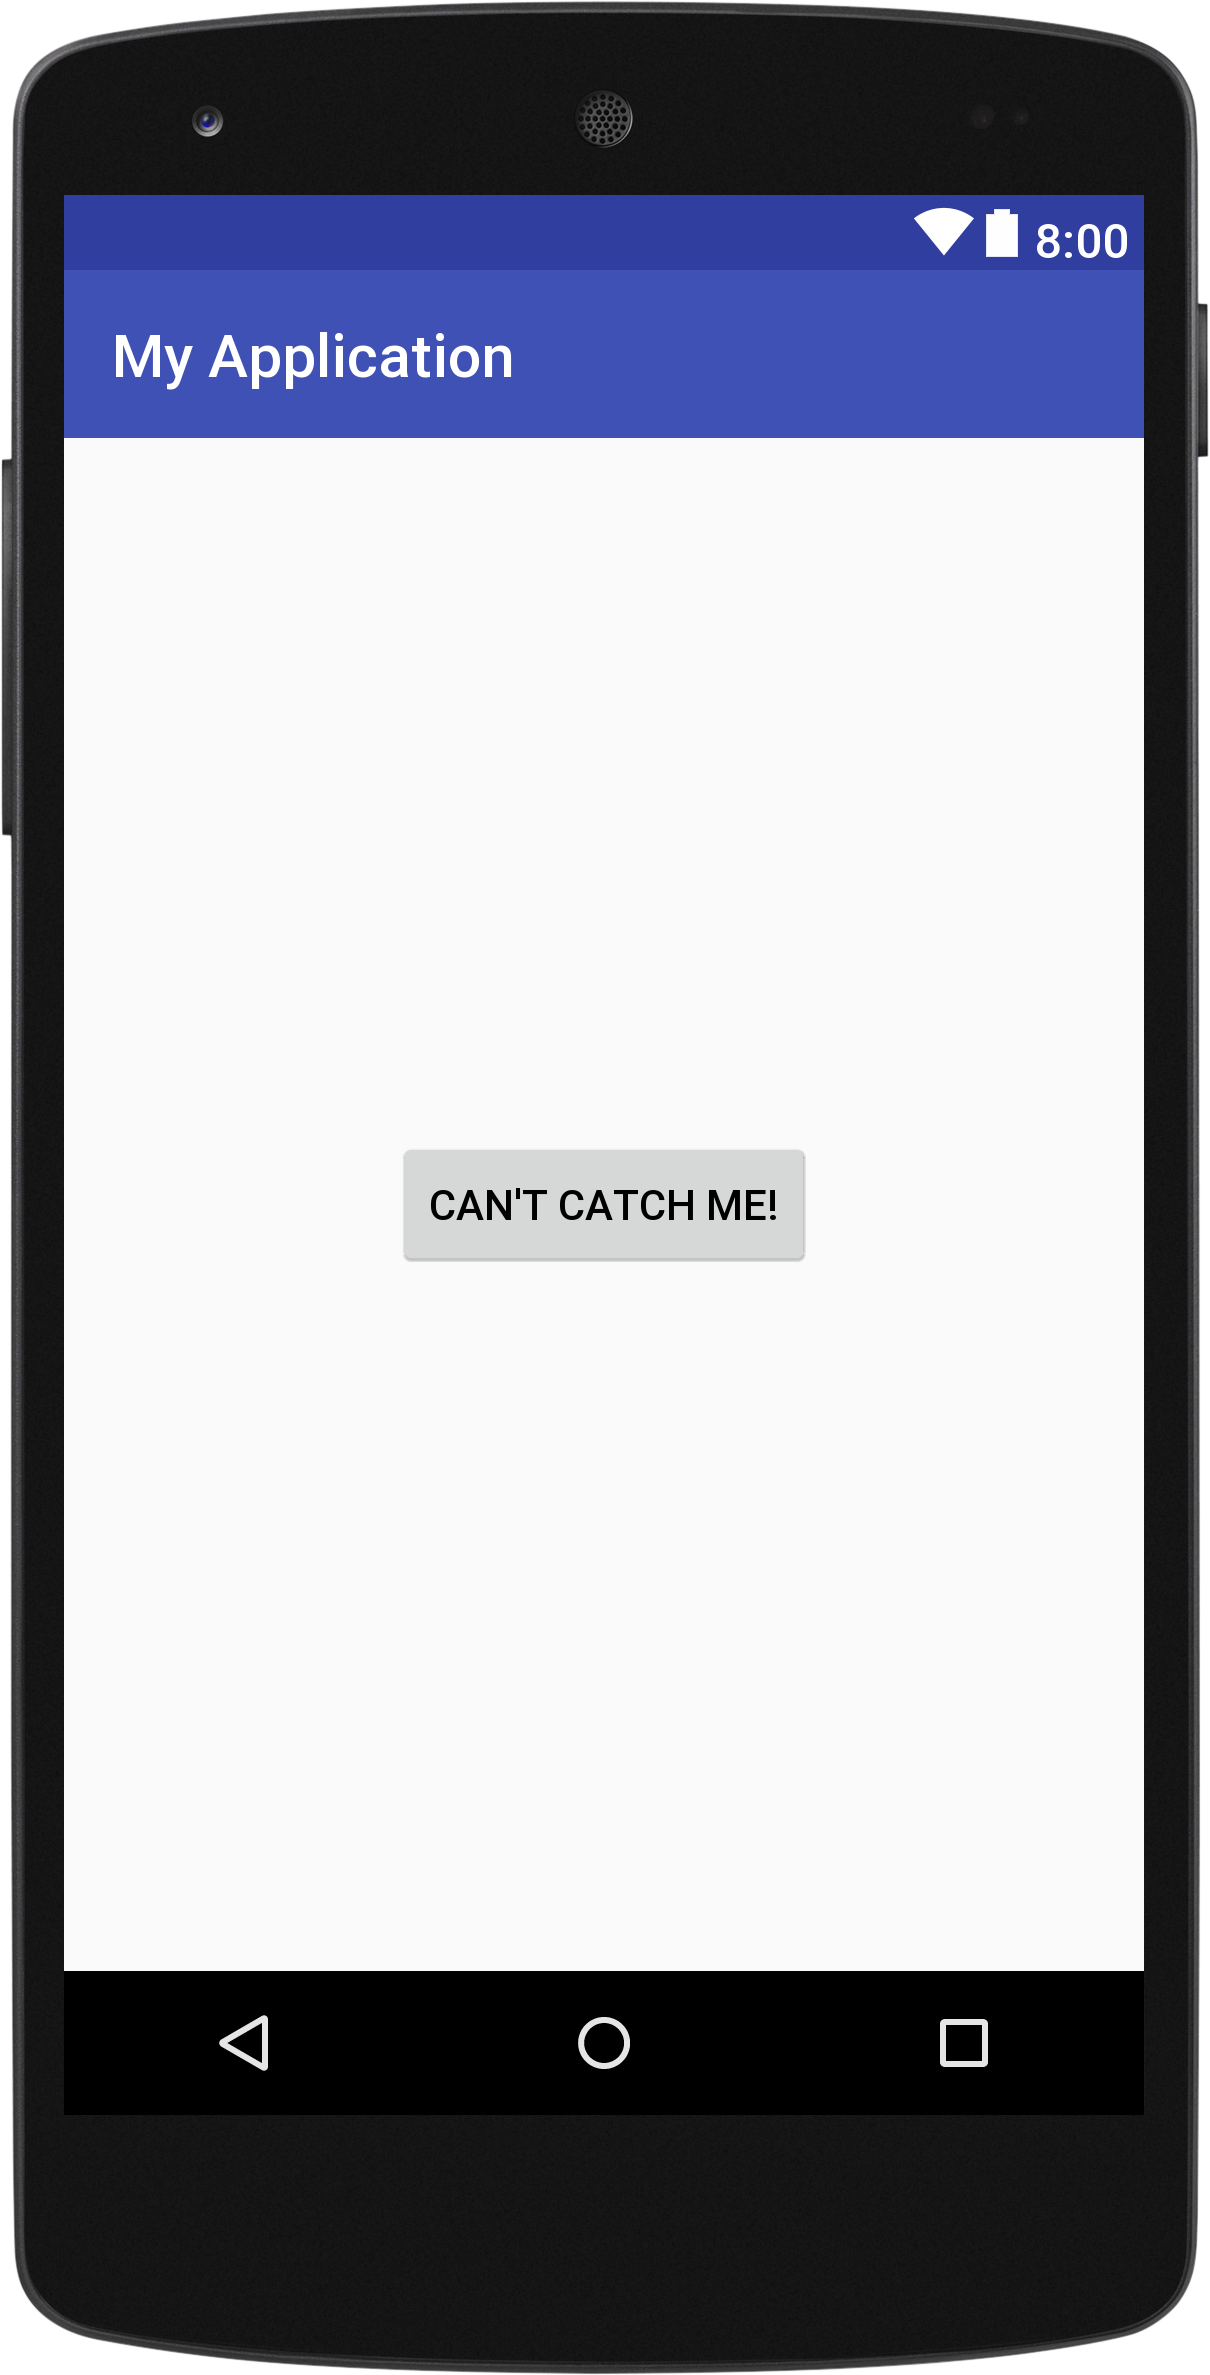
\includegraphics[width=5cm]{button_layout.png}
		\caption{Et relative layout med en knap i midten}
		\label{fig:android:layouts:button-layout}
	\end{center}
\end{figure}

Hvis vi nu gerne vil have at app'en reagerer på at vi trykker på denne knap, så 
kan vi tilføje ``android:onClick'' attributten til knappen og give den attribut 
en værdi der svarer til den funktion vi gerne vil have til at køre når vi 
trykker på knappen. Et eksempel på dette kan ses i \autoref{lst:button-layout}.
Herefter kan vi blot tilføje den funktion vi tilføjede i ``onClick'' 
attributten til vores activity, som vist i \autoref{lst:button-activity}.

Vi kan se at ``buttonClicked'' funktionen får et ``View'' med som argument. 
Dette View er det element i app'ens \gls{interface} der har udløst funktionen. 
I dette tilfælde er det knappen man trykkede på. Hvis vi lægger $10$ til dens 
$x$ værdi, vil den flytte sig $10$ ``pixels'' til højre.

\begin{exercise}
	Implementer layoutet beskrevet i \autoref{lst:button-layout} og aktiviteten 
	i \autoref{lst:button-activity}.
\end{exercise}

\begin{exercise}
	Hvorfor skal vi lægge noget til $x$ for at flytte knappen mod højre? Hvad 
	betyder $x$?
\end{exercise}

\begin{exercise}
	Hvordan flytter man i stedet knappen op, ned eller til venstre?
\end{exercise}

\begin{exercise}
	Lav et layout med to knapper, den ene skal flytte sig op når man trykker, 
	den anden skal flytte sig mod højre.
\end{exercise}

\clearpage


\begin{XmlCode}{Et layout med en knap der kalder ``buttonClicked'' funktionen% 
når den bliver trykket på.}{lst:button-layout}
	<?xml version="1.0" encoding="utf-8"?>
	<RelativeLayout 
		xmlns:android=
			"http://schemas.android.com/apk/res/android"
		xmlns:tools="http://schemas.android.com/tools"
		android:layout_width="match_parent"
		android:layout_height="match_parent"
		tools:context=
			"com.example.lukas.myapplication.MainActivity">
	
	<Button
		android:id="@+id/catchMeButton"
		android:layout_width="wrap_content"
		android:layout_height="wrap_content"
		android:layout_centerInParent="true"
		android:onClick="buttonClicked"
		android:text="Can't catch me!" />
		
	</RelativeLayout>
\end{XmlCode}

\clearpage

\begin{JavaCode}{En activity der flytter en knap nedad når den bliver trykket %
på.}{lst:button-activity}
	public class MainActivity extends AppCompatActivity {
		
		@Override
		protected void onCreate(Bundle savedInstanceState) {
			super.onCreate(savedInstanceState);
			setContentView(R.layout.activity_main);
		}
		
		
		public void buttonClicked(View view) {
			view.setX(view.getX() + 10);
		}
	}
\end{JavaCode}


